\documentclass[14pt,handout]{beamer}
%aspectratio=169
\usepackage[utf8]{inputenc}
\usepackage[T1]{fontenc}
\usepackage[magyar]{babel}
\usetheme{default}
%\usepackage{enumitem} %settings of itemize, e.g. itemsep


\title{Korszerű fűtési rendszerek szabályozása}
\author{Gyulai László}
%\institute{Szakdolgozat bemutatás}
\date{2019. január 7.}

\newcommand\Fontvi{\fontsize{6}{7.2}\selectfont}


\usepackage{graphicx}
\usepackage{tikz}
\usetikzlibrary{mindmap,trees}
\usepackage{verbatim}

%\begin{document}
%	\pagestyle{empty}
	
	\begin{comment}
	:Title: Computer science mindmap
	:Tags: Manual, Mindmap
	
	Version 1.09 of PGF/TikZ added a library for drawing mindmaps. Here's an example
	from the manual. 
	
	| Author: Till Tantau
	| Source: The PGF/TikZ manual
	
	\end{comment}
	%\end{document}

\begin{document}
	
	\frame{\titlepage}
\begin{frame}{Bevezető}

%[shrink=-25]
    \begin{itemize}
        \item Témaválasztás szempontjai
        \pause
        \setlength{\itemsep}{6pt}
        \begin{itemize}
            \item szabályozástechnikai vonatkozás
            \item gyakorlati haszon, piaci igény 
        \end{itemize}
    	\pause
    	\item \underline{Korszerű fűtési rendszerek szabályozása}
    	\pause
        \begin{itemize}
            \setlength{\itemsep}{3pt}
        	\item a fenti kívánalmaknak megfelel
        	        	
	    	\item a témában érintett szakterületek:
	    	\pause
	        \begin{itemize}
	            \item Épületgépészet
	            \item Szabályozástechnika
	            \item Jogszabályok, pénzügy és marketing 
	            %környezetgazdaságtan
	        \end{itemize}
        \end{itemize}
    \end{itemize}

\end{frame}

\begin{frame}{A munka célja}
\begin{itemize}
	\setlength{\itemsep}{6pt}
	\item Szabályozástechnikai tudás elményítése
	\item Kutatási eredmények megismerése
	\item Mindeközben törekvés a piacképességre is	
\end{itemize}
\end{frame}




%\begin{frame}{Műszaki tartalom}
%\Fontvi
%\centering
%\begin{tikzpicture}[thick,scale=0.7, every node/.style={scale=0.7}]
%\path[mindmap,concept color=black,text=white]
%node[concept] {\normalsize Termékfejlesztés}
%[clockwise from=-30]
%child[concept color=green!50!black] {
%	node[concept] {Tudás-\\vezérelt\\ötlet}
%	[clockwise from=0]
%	child { node[concept] {épületfizika} }
%	child {
%		node[concept] {szabályozástechnika}
%		[clockwise from=-45, level 3 concept/.append style={sibling angle=50, thick,scale=1.1}]
%		child { node[concept] {MIMO\\rendszerek} }
%		child { node[concept, scale=1.2] { \scalebox{0.9}{prediktív}\\ \scalebox{0.9}{szabályozás}} }
%	}
%	%child { node[concept] {pro\-gramming languages} }
%}  
%child[concept color=blue] {
%	node[concept] {applied}
%	%	[clockwise from=-30]
%	%	child { node[concept] {databases} }
%	%	child { node[concept] {WWW} }
%}
%child[concept color=red] {
%	node[concept] {Piacvezérelt\\ ötlet}
%	[clockwise from=-90]
%	child { node[concept] {törvényi \\ előírások} }
%	child { node[concept] {piaci \\ igények} }
%};
%\end{tikzpicture}
%\end{frame}
%
%
%
%
%\begin{frame}{Műszaki tartalom}
%\Fontvi
%\centering
%\begin{tikzpicture}[thick,scale=0.65, every node/.style={scale=0.65}]
%\path[mindmap,concept color=black,text=white]
%node[concept] {\normalsize Termékfejlesztés}
%[clockwise from=150, level 1 concept/.append style={sibling angle=120}]
%
%child[concept color=red] {
%	node[concept] {Piacvezérelt\\ ötlet}
%	[clockwise from=-120, level 2 concept/.append style={sibling angle=120}]
%	child { node[concept] {törvényi \\ előírások} }
%	child { node[concept] {piaci \\ igények} }
%}
%child[concept color=green!50!black] {
%	node[concept] {Tudás-\\vezérelt\\ötlet}
%	[clockwise from=45, level 2 concept/.append style={sibling angle=100}]
%	child { node[concept] {épületfizika} }
%	child {
%		node[concept] {szabályozástechnika}
%		[clockwise from=60, level 3 concept/.append style={sibling angle=100, thick,scale=1.1}]
%		child { node[concept] {MIMO\\rendszerek} }
%		child { node[concept, scale=1.2] { \scalebox{0.9}{prediktív}\\ \scalebox{0.9}{szabályozás}} }
%	}
%	%child { node[concept] {pro\-gramming languages} }
%}
%child[concept color=blue] {
%	node[concept] {applied}
%	%	[clockwise from=-30]
%	%	child { node[concept] {databases} }
%	%	child { node[concept] {WWW} }
%};
%\end{tikzpicture}
%\end{frame}



\begin{frame}{Műszaki tartalom}
\Fontvi
\centering
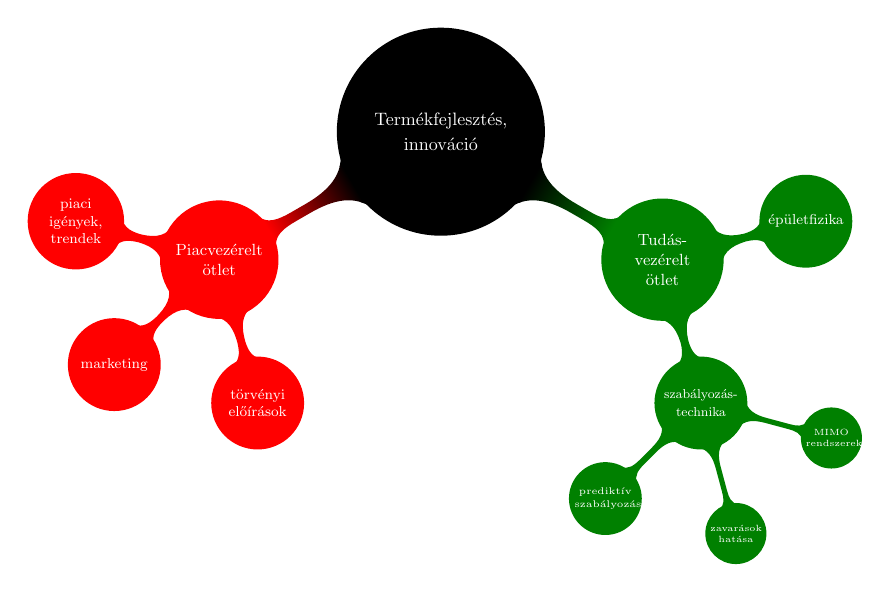
\begin{tikzpicture}[thick,scale=0.65, every node/.style={scale=0.65}]
\path[mindmap,concept color=black,text=white]
node[concept] {\normalsize Termékfejlesztés,\\innováció}
[counterclockwise from=210, level 1 concept/.append style={sibling angle=120}]

child[concept color=red] {
node[concept] {Piacvezérelt\\ ötlet}
[clockwise from=-75, level 2 concept/.append style={sibling angle=60}]
child { node[concept] {törvényi \\ előírások} }
child { node[concept] {marketing} }
child { node[concept] {piaci \\ igények,\\trendek} }
}
child[concept color=green!50!black] {
node[concept] {Tudás-\\vezérelt\\ötlet}
[clockwise from=15, level 2 concept/.append style={sibling angle=90}]
child { node[concept] {épületfizika} }
child {
	node[concept] {\scalebox{0.9}{szabályozás-}\\ \scalebox{0.9}{technika}}
	[clockwise from=-15, level 3 concept/.append style={sibling angle=60, thick,scale=1.1}]
	child { node[concept] {MIMO\\rendszerek} }
	child { node[concept] {zavarások\\hatása} }
	child { node[concept, scale=1.2] { \scalebox{0.9}{prediktív}\\ \scalebox{0.9}{szabályozás}} }
}
%child { node[concept] {pro\-gramming languages} }
};
\end{tikzpicture}
\end{frame}

\begin{frame}{Műszaki tartalom}

Piacvezérelt vagy tudásalapú terméket szeretnék?

\begin{itemize}
	\setlength{\itemsep}{7pt}
	\item tudományos: korszerű szabályozások, pl.
	\begin{itemize}
		\item optimális
		\item prediktív
		\item robosztus%szabályozástechnikai ismeretekre van szükség
	\end{itemize}
	\item piacvezérelt: igények alapján
	\begin{itemize}
		\item PI-szabályzós termosztát (önhangoló)
		\item intelligens otthonok (marketinggel fűszerezve)
	\end{itemize}
\end{itemize}
\end{frame}


\begin{frame}{Műszaki tartalom}

Piacvezérelt vagy tudásalapú terméket szeretnék?

\begin{itemize}
	\setlength{\itemsep}{7pt}
	\item Modellalapú szabályozás
	\begin{itemize}
		\item nagyobb komfort, alacsonyabb költségek
		\item innovatív, kutatják, publikálják az eredményeket
		\item komplex modellek, MIMO rendszerek kezelése
		\item optimalizációra visszavezethető beavatkozás\footnote{Az optimális beavatkozásnak sokféle kritériuma lehet.}
		%\item fontosabb a szabályozás minősége, mint hogy univerzális legyen
		%\item mérhető és nem mérhető zavarások figyelembe vétele
	\end{itemize}
	\item Kiindulás a piacon elérhető megoldásokból
	\begin{itemize}
		\item felkapott: intelligens otthon rendszerek
		\item multicégek termékei: Siemens, Bosch, Johnson Controls, Honeywell, Danfoss termosztátjai, okos rendszerei
		%\item fontosabb a szabályozás minősége, mint hogy univerzális legyen
		%\item mérhető és nem mérhető zavarások figyelembe vétele
	\end{itemize}
\end{itemize}
\end{frame}

\begin{frame}{Piacvezérelt termékfejlesztés}

Mire van igény a piacon?

\begin{itemize}
	\setlength{\itemsep}{7pt}
	\item Van egy problémakör:
	\begin{itemize}
		\item energiahatékonyság (törvényi megfelelőség)
		\item nagy kibocsátás
		\item magas költségek
		\item diszkomfort
	\end{itemize}
	\pause
	
	\item Megoldási lehetőség:
	\begin{itemize}
		\item egy korszerű fűtésszabályozás,\\
		ami teljesíti a követelményeket?
		%\item intelligens otthonok (marketinggel fűszerezve)
	\end{itemize}
\end{itemize}
\end{frame}



\begin{frame}{Tudásalapú termékfejlesztés}

Mit szeretnék csinálni?
\pause
\vspace{6pt}

\begin{itemize}
	\setlength{\itemsep}{12pt}
	\item Szabályozástechnika (analízis és tervezés):
	\begin{itemize}
		\item MIMO rendszerek paraméterbizonytalansággal
		\item mérhető vagy becsülhető zavarások
		\item prediktív szabályozás
	\end{itemize}
	\pause

	\item Fejlesztési lehetőség:
	\begin{itemize}
		\item egy korszerű fűtésszabályozás, \\
		amivel a fentiek vizsgálhatók, szemléltethetők?
		%\item intelligens otthonok (marketinggel fűszerezve)
	\end{itemize}
\end{itemize}
\end{frame}

\begin{frame}{A kiválasztott irány}

Szabályozástechnikai feladat:

\begin{itemize}
	\item helyiségenkénti hőmérsékletszabályozás,
	\item radiátoros és padlófűtéssel
\end{itemize}
\vspace{6pt}

Ehhez szükséges:


\begin{itemize}
	\item a szakasz paraméterezhető modellje
	\item egy modell-prediktív szabályozó
\end{itemize}


\end{frame}


\begin{frame}{MPC szabályozás}

Publikációk alapján a leggyakoribb korszerű szabályozó

\begin{itemize}
	\setlength{\itemsep}{12pt}
	\item Modellalapú működés - kép a Simulinkből
	\begin{itemize}
		\item épület
		\item fűtési rendszer
		\item prediktív szabályozás
	\end{itemize}
	\item Követelményei:
	\begin{itemize}
		\item radiátorszelep
		\item hőmérő
	\end{itemize}
\end{itemize}
\end{frame}



\begin{frame}{Szimuláció, modellalkotás}

A modell nagyon részletesen szerepel a dolgozatban, elvi újdonságot nem tartlalmaz (RC-hálózat) és a szabályozás rész érdekesebb, azzal foglalkoznék.

Tervezés szimulációval.

%\begin{itemize}
%\setlength{\itemsep}{10pt}
%\item Szabályozástechnika (analízis és tervezés):
%\begin{itemize}
%	\item MIMO rendszerek paraméterbizonytalansággal
%	\item mérhető vagy becsülhető zavarások
%	\item prediktív szabályozás
%\end{itemize}
%\item Fejlesztési lehetőség:
%\begin{itemize}
%	\item egy korszerű fűtésszabályozás?
%	%\item intelligens otthonok (marketinggel fűszerezve)
%\end{itemize}
%\end{itemize}


\end{frame}

\begin{frame}{Tervezés lépései}

Szimuláció:
\begin{itemize}
	\item valós rendszer modelljének paraméterezése
	\item modell identifikáció
	\item szabályozás tervezése, validálása
\end{itemize}
\vspace{6pt}

Valós rendszerre:
\begin{itemize}
	\item a tervezett szabályozó kipróbálása
	\item finomítás
\end{itemize}

\end{frame}




\begin{frame}{Műszaki tartalom2}
\Fontvi
\centering
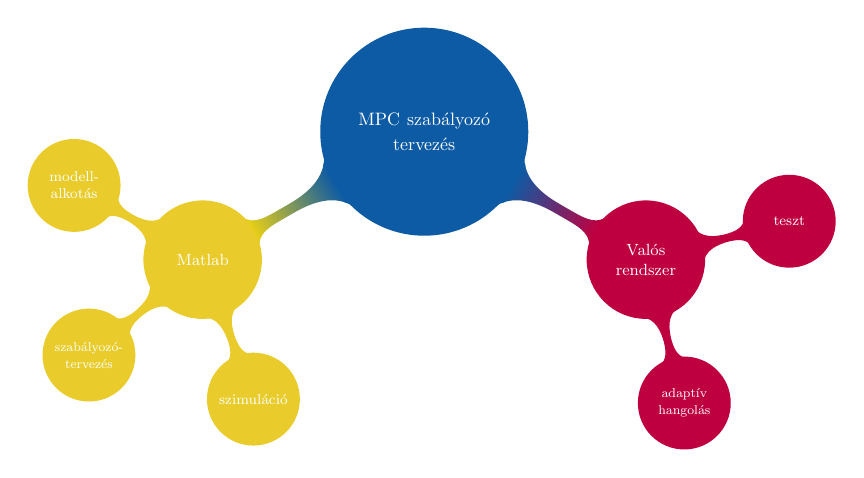
\begin{tikzpicture}[thick,scale=0.65, every node/.style={scale=0.65}]
%\tikzset{level 1 concept/.append style={level distance = 90mm, scale=0.5}}
\path[mindmap,concept color=blue!66!green!90!gray,text=white]
node[concept] {\normalsize MPC szabályozó\\tervezés}
[counterclockwise from=210, level 1 concept/.append style={node distance=6cm,sibling angle=120}]

child[concept color=yellow!80!gray!90!red] {
	node[concept] {Matlab}
	[clockwise from=-70, level 2 concept/.append style={sibling angle=70}]
	child { node[concept] {szimuláció} }
	%child { node[concept] {energetikai\\tanúsítvány} }
	child { node[concept] {\scalebox{0.9}{szabályozó-}\\ \scalebox{0.9}{tervezés}} }
	child { node[concept] {modell-\\alkotás} }
}
child[concept color=blue!25!red] {
	node[concept] {Valós rendszer}
	[clockwise from=15, level 2 concept/.append style={sibling angle=90}]
	child { node[concept] {teszt} }
	child {
		node[concept] {\scalebox{0.9}{adaptív}\\ \scalebox{0.9}{hangolás}}
		[clockwise from=-15, level 3 concept/.append style={sibling angle=60, thick,scale=1.1}]
		%child { node[concept] {historikus\\adatok} }
		%child { node[concept, scale=1.2] { \scalebox{0.9}{prediktív}\\ \scalebox{0.9}{szabályozás}} }
	}
	%child { node[concept] {pro\-gramming languages} }
};
\end{tikzpicture}
\end{frame}



\end{document}
